\section{Design}
\subsection{Modules and Data Flow}
Input handling turns stable presses and accepted coins into events. The state
controller stores credit, the cycle start time and the STOP count. The timer checks
elapsed time. Output logic sets both LEDs and the wash enable signal.
\fig{01_module_diagram.pdf}{0.90}{Main modules and their data flow.}

\subsection{State Machine}
Use five states: Standby, Ready, Running, Paused and Error.
Figure~\ref{fig:fsm} shows the main transitions. Coin collection below
50 cents stays in Standby.
\begin{figure}[H]\centering
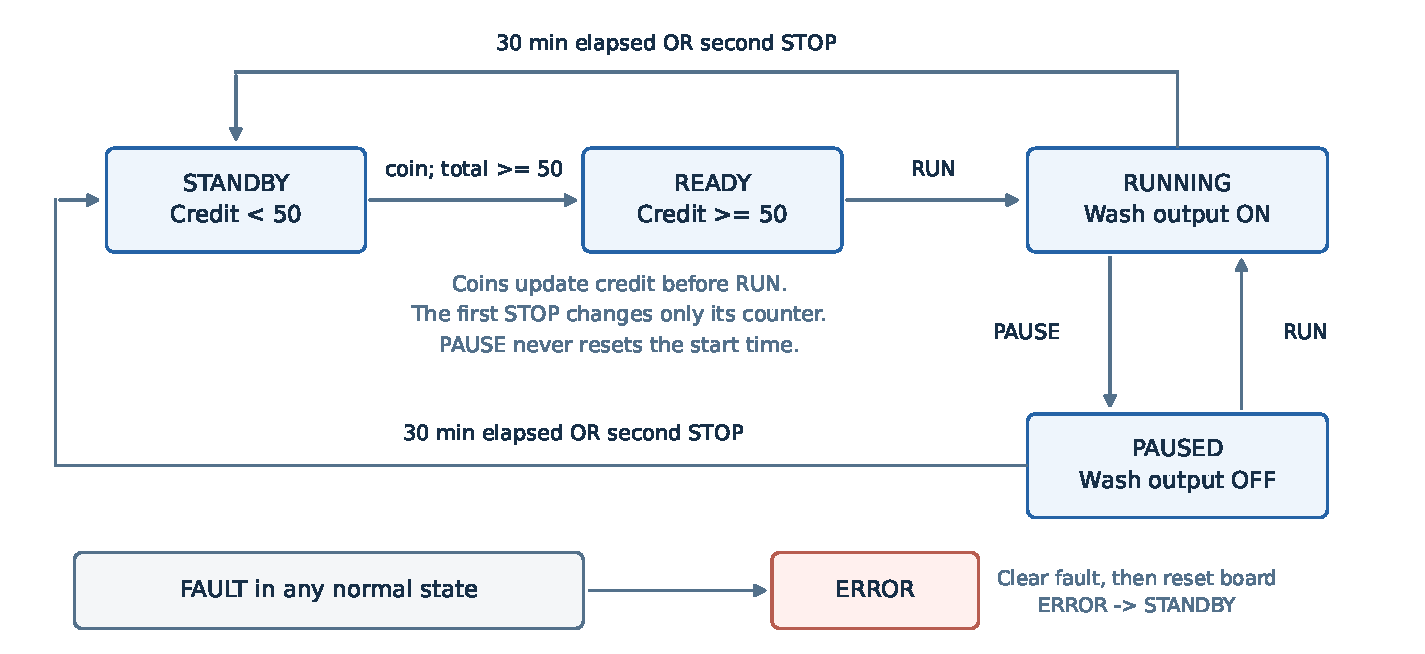
\includegraphics[width=0.92\linewidth]{figures/02_state_diagram.pdf}
\caption{Main state transitions. A fault can enter Error from any normal state.}
\label{fig:fsm}
\end{figure}

\subsection{Outputs in Each State}
\begin{tabularx}{\linewidth}{@{}p{2.3cm}YYYp{3.05cm}@{}}
\toprule
State & RLED & BLED & Wash output & Timer\\
\midrule
Standby & On & Off & Off & Not active\\
Ready & On & On & Off & Not active\\
Running & Off & Blink & On & Counting\\
Paused & Off & On & Off & Counting\\
Error & Blink & Off & Off & Cycle cancelled\\
\bottomrule
\end{tabularx}
Blink means 500 ms on and 500 ms off. The ready and paused combinations follow
the explicit choices in Section 1.2.
